\clearpage
\section{W Polarisation Closure Test\label{app:wpol}}

As the LHC is a pp collider, high $p_T$ W bosons are predominantly
produced left handed \cite{WPol}.  For high $p_T$ bosons, this implies
that $W^+$ will decay to the left handed neutrino along its direction
of motion while the lepton will be backward. The opposite behaviour is
expected for the $W^-$. The lepton will therefore be more boosted (and
the neutrino less boosted) in $W^+$ decays than $W^-$ decays.  This
leads to a larger number of $W^+$ decays in the single lepton control
regions (which relies on the lepton $p_T$ for acceptance) than in the
signal region (which relies on the neutrino $p_T$ for acceptance). In
order to understand if this leads to a bias in the prediction of the
$W$ and unpolarised \zInv\ background in the signal region when using
a single lepton control region a closure test from $\mu^+$ + jets to
$\mu^-$ + jets will be added.  The \mj to \mmj abd \mj to \gj closure 
tests will also be important for probing the effect in the \zInv\ prediction. 
The results from these closure tests using $8\TeV$ data can be seen in
Figure~\ref{fig:wpolCT}.  No significant bias or trend is observed.

\begin{figure}[h!]
 \begin{center}  
  \subfigure[Closure tests for $\le3$ jets]{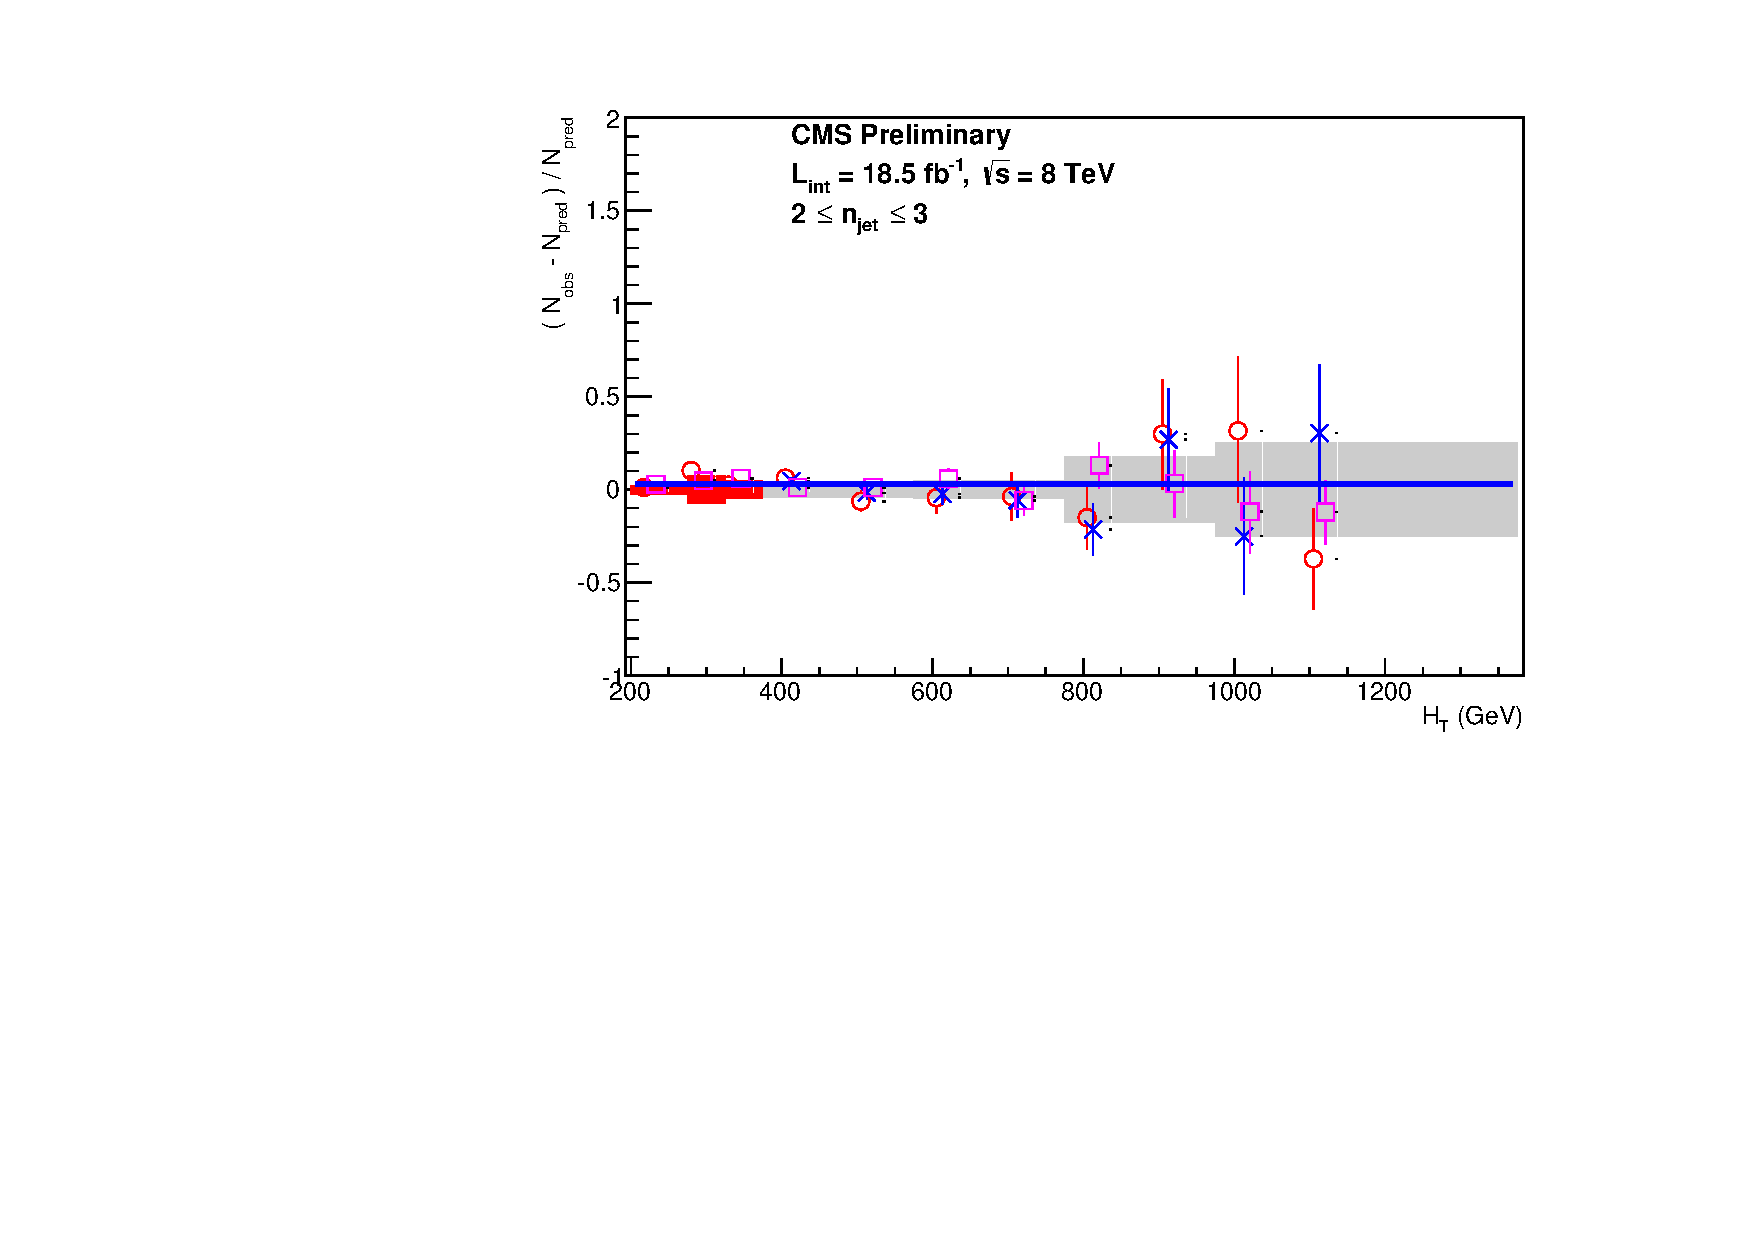
\includegraphics[width=0.5\textwidth]{figures/wPol/summaryLe3J.pdf}} ~~
  \subfigure[Closure tests for $\ge4$ jets]{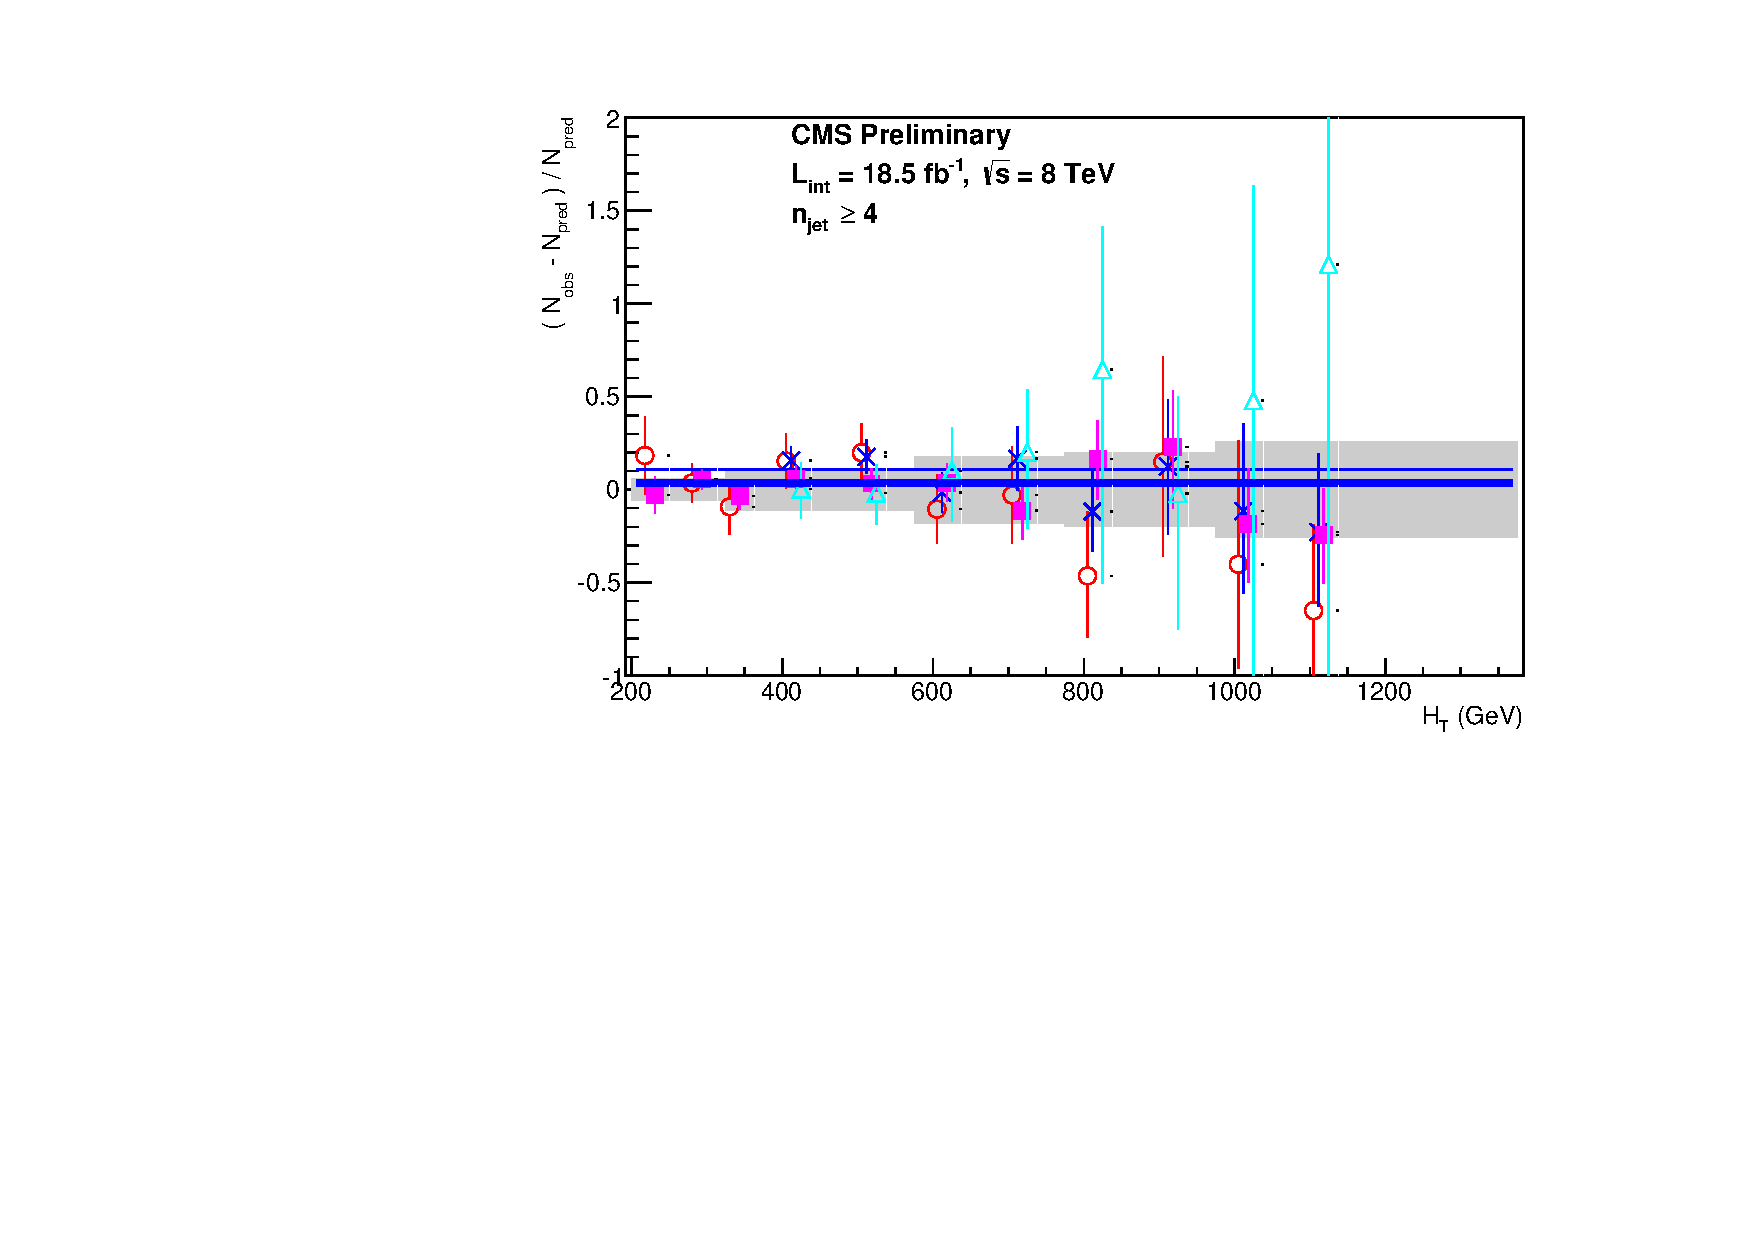
\includegraphics[width=0.5\textwidth]{figures/wPol/summaryGe4J.pdf}}
  \caption{Closure tests that probe the effects of W polarisation on
    experimental acceptance. The red circles correspond to the \mj to
    \mmj closure test, the blue crosses correspond to the \mj to \gj closure test
     and the pink squares correspond to the
    $\mu^+$ + jets to $\mu^-$ + jets closure test.}
  \label{fig:wpolCT}
 \end{center}
\end{figure}          
